% -*- coding: utf-8 -*-
%%
%%  本模板可以使用以下两种方式编译:
%%     1. PDFLaTeX
%%     2. XeLaTeX [推荐]
%%  注意:
%%    1. 在改变编译方式前应先删除 *.toc 和 *.aux 文件,
%%       因为不同编译方式产生的辅助文件格式可能并不相同。

%\documentclass{cumcmart}
\documentclass[nocover]{cumcmart}%%%切换到无封面的版本,有些区域不允许前面的承诺页用pdf格式,可以用此去掉。



\begin{document}

\xuanti{A}
%\school命令用于在承诺书上显示学校名称。按要求,此处应填写全称
\school{长江大学}
%以下命令分别显示队员及指导教师姓名
\numbers{2017000}%参赛报名号
\authorone{成员一}
\authortwo{成员二}
\authorthree{成员三}
\advisor{数模指导组}

%\theyear{2017}
\theday{11}%填写当月的具体日期

\title{根据太阳影子定位}
\maketitle

% \begin{cnabstract}%此处没有采用sbstract命名,是为了将来如果要加入英文摘要时扩展的方便


% \cnkeywords{差分方程,元胞自动机,交通阻塞模型,数值模拟}
% \end{cnabstract}

% \newpage
%\tableofcontents\newpage%增加目录,要不要都可以。不想要的话,就在本行前加“%”(英文的百分号)


\section{问题重述}

随着现代社会科技水平的不断提高和通信技术的愈加完善,定位技术受到了越来越多的关注。太阳影子定位技术就是通过分析视频中物体的太阳影子变化,确定视频拍摄的地点和日期的一种方法。根据附件,解决以下问题:
\begin{enumerate}
\item 建立影子长度变化的数学模型,分析影子长度关于各个参数的变化规律,并应用你们建立的模型画出2015年10月22日北京时间9:00-15:00之间天安门广场(北纬39度54分26秒,东经116度23分29秒)3米高的直杆的太阳影子长度的变化曲线;
\item 根据某固定直杆在水平地面上的太阳影子顶点坐标数据,建立数学模型确定直杆所处的地点。将你们的模型应用于附件1的影子顶点坐标数据,给出若干个可能的地点;
\item 根据某固定直杆在水平地面上的太阳影子顶点坐标数据,建立数学模型确定直杆所处的地点和日期。将你们的模型分别应用于附件2和附件3的影子顶点坐标数据,给出若干个可能的地点与日期;
\item 附件4为一根直杆在太阳下的影子变化的视频,并且已通过某种方式估计出直杆的高度为2米。请建立确定视频拍摄地点的数学模型,并应用你们的模型给出若干个可能的拍摄地点。如果拍摄日期未知,你能否根据视频确定出拍摄地点与日期?
\end{enumerate}

\section{建模分析}

\subsection{模型假设}
针对该问题,我们提出了如下的合理假设:
\begin{enumerate}
\item 地球为均匀球体;
\item 忽略大气折射作用,即太阳光线平行照射地球;
\item 
\item 
\end{enumerate}

\subsection{记号说明}
\begin{table}[!htbp]
    \centering
    \begin{tabular}{cl}
    \toprule
    \multicolumn{2}{c}{\large 模型记号说明}\\
    \midrule
        $h$           & 太阳高度角 \\
        $\phi$        & 观测地地理纬度  \\
        $\delta$      & 太阳赤纬角  \\
        $t$           & 地方时(时角) \\  
        $A$           & 太阳方位角 \\
        $H$          & 直杆长度  \\
        $l$          & 影子长度  \\
    \bottomrule
    \end{tabular}
    \caption{模型记号说明}
\end{table}

\subsection{问题分析}
对于问题一,我们已知直杆的长度为 米高,根据物理光学的知识,如果我们再知道平行光源的入射角,就可以知道影子的长度。但实际情况是,由于太阳光线的入射角(高度角)是随时间变化的,也导致影子的长度随时间变化,这样就可以转化为影子的长度随时间的变化规律
\subsection{模型求解和分析}
由太阳高度角公式: $ \sin(h) = \sin(\phi)sin(\delta)+\cos(\delta)cos(\phi)\cos(t)$,可以知道太阳高度角主要由当地的地理纬度、季节(日、月)和时间三个因素决定的,分别计算出各值即可求出太阳高度角随时间的变化。

\subsection{模型评价}
\subsubsection{模型优点}
1)	

2)	

3)	

\subsubsection{模型缺点}
1)	

2)	


%   \begin{figure}
%   \centering
%   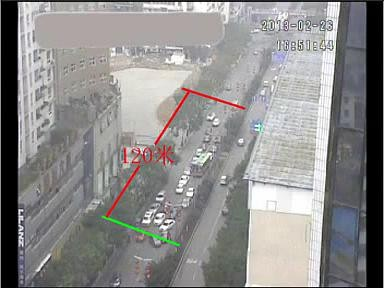
\includegraphics[width=.6\textwidth]{fig1}
%   \caption{发生事故时车流饱和状态图示}
%   \end{figure}

% \begin{thebibliography}{10}
% \bibitem{1} \url{http://bbs.chinatex.org}
% \bibitem{2} \url{http://www.chinatex.org}
% \bibitem{3} Alpha Huang, \textbf{latex-notes-zh-cn}, 2014.
% \bibitem{lf}M.R.C. van Dongen,\textbf{\LaTeX-and-Friends}, 2013.
% \bibitem{figure}Keith Reckdahl,\textbf{Using Import graphics in \LaTeXe}, 1997.
% \bibitem{HM}Addison Wesley,\textbf{Higher Mathematics}, 下载地址如下\\ \url{http://media.cism.it/attachments/ch8.pdf}
% \end{thebibliography}


\newpage
\appendix
\section*{附 \quad 录}

\section{matlab 源程序}
\begin{lstlisting}
\lipsum[13]

\textbf{\textcolor[rgb]{0.98,0.00,0.00}{Input matlab source:}}
\lstinputlisting[language=Matlab]{./code/mcmthesis-matlab1.m}


\end{lstlisting}


\end{document}
